\chapter{Data and Preprocessing}
\label{chap:data-and-preprocessing}
\section{Datasets: NLST and DLCSD24}
The development and evaluation of computer-aided detection systems for pulmonary nodules heavily rely on comprehensive and diverse datasets. In this work, we leverage two distinct datasets: the National Lung Screening Trial (NLST) \cite{nlst_data} and the Duke Lung Cancer Screening Dataset 2024 (DLCSD24) \cite{dlcsd24}. Each dataset presents unique several slices/volumes of CT scans, annotated with pulmonary nodule locations, necessary for training and validating our detection models.

Both datasets will serve as 2D datasets, meaning that each slice of the CT scan will be treated as a separate image. The slicing will be done along the axial plane, which is the most common orientation for viewing CT scans.
The NLST dataset already comes as a collection of 2D slices on the axial plane, while the DLCSD24 dataset comes as a collection of 3D volumes that will need to be sliced along our desired plane, and possibly only a subset of slices of interest -- namely those containing nodules -- will be retained for training and evaluation.

\subsection{National Lung Screening Trial (NLST)}
The NLST is a large-scale, randomized controlled trial conducted by the National Cancer Institute (NCI) to determine if spiral computed tomography (CT) screening could reduce lung cancer mortality compared to standard chest X-ray. It enrolled over 53,000 participants at 33 sites across the United States. For the purpose of this study, the NLST dataset provides a vast collection of low-dose CT scans, which are invaluable for training nodule detection models.
Unfortunately, only a small subset of the NLST dataset includes annotations for pulmonary nodules, and these only cover malignant nodules.
After this filtering, we are left with approximately 9000 scans, each containing on average one nodule, for a total of around 9000 nodules of size greater or equal to 4 mm.
Regardless the absence of benign annotations, the NLST can be effectively utilized to teach a model to recognize nodule-like structures. Furthermore, the NLST dataset can serve as an excellent source for pre-training detection models, allowing them to learn general features of pulmonary nodules before fine-tuning on datasets with more detailed annotations.


\subsection{Duke Lung Cancer Screening Dataset 2024 (DLCSD24)}
The Duke Lung Cancer Screening Dataset (DLCS 2024) is a large-scale, annotated collection of low-dose thoracic CT scans designed to support research in lung nodule detection and cancer risk assessment using modern CT technology \cite{dlcsd24}. The dataset was compiled from screening examinations conducted at the Duke University Health System between January 2015 and June 2021, and consists of 1,613 CT volumes drawn from a pool of 2,061 patients, with additional cases reserved for future releases. Within these scans, a total of 2,487 nodules were annotated through a semi-automated pipeline in which a detection model, pre-trained on the LUNA16 dataset, generated candidate nodules that were subsequently verified and refined using radiology reports and expert review. Manual adjustments were performed by a medical student and a fellowship-trained cardiothoracic radiologist, and independent spot checks confirmed that the resulting annotations achieved an accuracy exceeding ninety percent. The dataset is released in multiple parts, with versioned updates hosted on Zenodo to ensure accessibility and reproducibility, and represents the first publicly available, large-scale screening dataset acquired with up-to-date CT protocols. As such, DLCS 2024 provides a valuable benchmark for developing and evaluating artificial intelligence models for lung nodule detection and classification in contemporary clinical practice.
Compared to the NLST, the DLCSD24 dataset offers both malignant and benign nodule annotations, despite with a severe imbalance with a ratio of approximately 1:10. The nodules in this dataset are also generally smaller, a property that makes them more challenging to detect. The DLCSD24 dataset is therefore particularly well-suited for training and evaluating nodule detection models, as it provides a more comprehensive representation of the types of nodules that may be encountered in clinical practice.

\subsubsection{Slice Extraction from 3D Volumes}
The DLCSD24 dataset is provided as a collection of 3D CT volumes. As previously stated in this chapter, we want to extract a 2D dataset from these volumes by slicing them along the axial plane. This is done by iterating through each volume, and extracting each slice as a separate image. If we were to extract all slices, we would end up with an extremely large dataset, with the majority of the data being non-informative, as most slices do not contain any nodules. To mitigate this, we use the provided annotations to identify slices that contain nodules, and only retain those slices for our 2D dataset. This results in a more manageable dataset size, while still retaining the most relevant information for nodule detection. 

\begin{figure}[h]
    \centering
    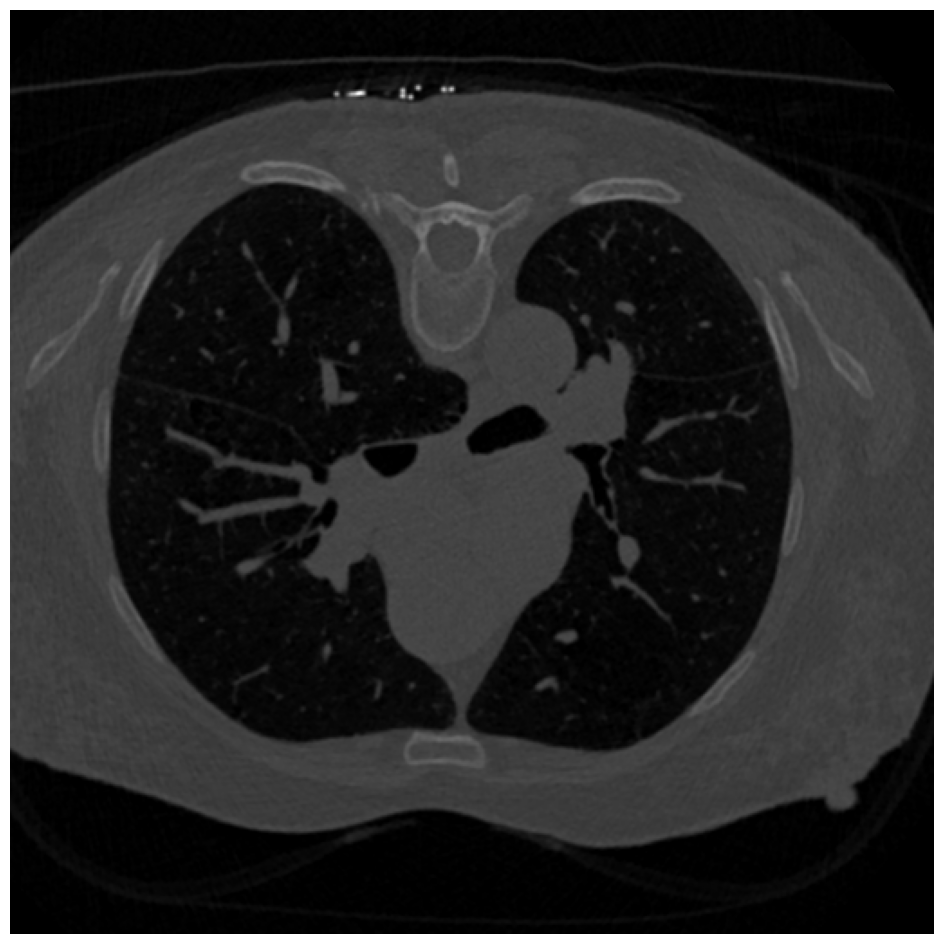
\includegraphics[width=0.6\linewidth]{images/dlcs_sample_unprocessed.png}
    \caption{Example of an unprocessed slice extracted from the DLCSD24 dataset.}
    \label{fig:dlcs-sample-unprocessed}
\end{figure}

% The size of the resulting 2D dataset depends on the thickness of the slices in the original 3D volumes, but in order to have a consistent size across all scans, we resample all volumes to have a slice thickness of 1.25mm, height and width spacing of 0.7mm, and then extract all slices containing nodules, along with a few slices before and after each nodule-containing slice to provide some context. This results in a final dataset of approximately 10,000 slices, each containing at least one nodule.

% This resampling step is crucial, as it ensures that all slices have the same resolution and spacing, which allows models to have a consistent spatial understanding of the images. 


\section{Preprocessing Pipeline}
\label{sec:preprocessing}
% Resampling, and HU clipping, explaining why we're clipping and why those ranges and not others, this is supported by the HU table.
% We might include here also discarded preprocessing steps, such as outlier removal (although it was a post-process step), and lung masking through morphological operations.

The preprocessing pipeline is a crucial step in preparing the CT scan data for effective analysis and model training. This pipeline involves several steps, including resampling, normalization, and Hounsfield Unit (HU) clipping, each of which plays an significant role in enhancing the quality and consistency of the input data and therefore quality of the detection.

\subsubsection{Resampling}
\label{sec:resampling}
CT scans can vary significantly in terms of their spatial resolution and slice thickness (a voxel might represent a differently sized parallelepiped in millimeters depending on the scan configurations), which can introduce inconsistencies when training machine learning models. To address this, we resample all CT scans to a uniform voxel (pixels for the NLST dataset) size of 1.25mm in the axial direction and 0.7mm in the coronal and sagittal directions.
These sizes were chosen according to \cite{tushar2025ailunghealthbenchmarking} as they represent a good compromise between preserving anatomical detail and managing computational resources.
This resampling is performed using bilinear interpolation, which helps to maintain the integrity of the anatomical structures while ensuring that all scans have a consistent spatial resolution.
For the DLCSD24 dataset, this resampling is performed before the slice extraction step on the entire 3D volume. Such operation is performed usign the MONAI framework \cite{monai}.

As for the NLST dataset, since it is already provided as a collection of 2D slices, we only need to ensure that each slice has the correct in-plane resolution of 0.7mm. If any slice does not meet this requirement, it is resampled using bilinear interpolation to achieve the desired resolution and it has been performed using the SimpleITK library \cite{lowekamp2013simpleitk} to extract the slices metadata and resample using its built-in resampler. The output size, given the desired spacing, original size and current spacing, is computed as follows:
$$
\text{output\_size} = \left( \left\lfloor\frac{S_1 \cdot \delta_1}{\delta_1^\prime}\right\rceil, \left\lfloor\frac{S_2 \cdot \delta_2}{\delta_2^\prime}\right\rceil, 1 \right)
$$

Where \(S_i\) is the original size along dimension \(i\), \(\delta_i\) is the original spacing along dimension \(i\), and \(\delta_i^\prime\) is the desired spacing along dimension \(i\). The output size is rounded to the nearest integer to ensure that it represents a valid number of pixels. Since the NLST dataset is already 2D, the output size for the third dimension is set to 1 as a dummy value.

\paragraph{Ablation Study Design:}
To empirically validate the effectiveness of the resampling step, an ablation study was designed. The performance of the Faster R-CNN model will be compared across two experimental conditions: 
\begin{itemize}
    \item \textbf{Baseline:} The model trained on the original dataset without any resampling.
    \item \textbf{Resampled:} The model trained on the dataset after applying the resampling step.
\end{itemize}
For this experiments we used the EfficientNetV2-S backbone \cite{tan2020efficientnet} and the results of this ablation study are presented in Figure \ref{fig:resampling-ablation}.
\begin{figure}[h]
    \centering
    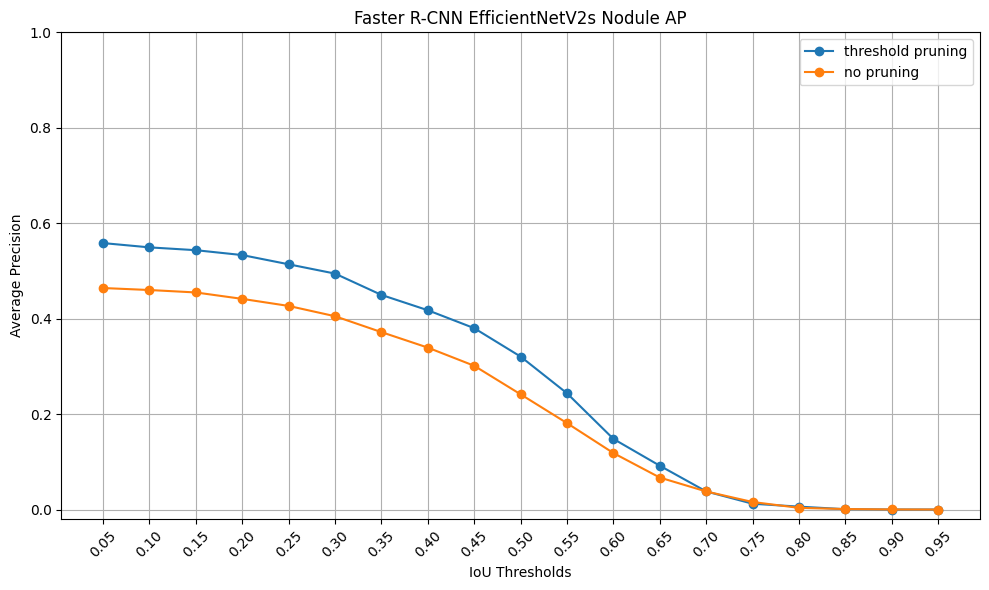
\includegraphics[width=0.8\linewidth]{images/resampling-ablation.png}
    \caption{Average Precision at varying IoU thresholds for the resampling ablation study.}
    \label{fig:resampling-ablation}
\end{figure}
As we can see from the results, the resampling step has a significant positive impact on the model's performance, particularly at higher IoU thresholds. This demonstrates the importance of having a consistent spatial resolution across all scans, validating the effectiveness of the resampling step in the preprocessing pipeline.

\subsubsection{Hounsfield Unit Clipping}
\label{sec:hu-clipping}
Hounsfield Units (HU) are a quantitative scale for describing radiodensity in medical CT imaging. Different tissues and materials in the body have characteristic HU values, which can be used to differentiate between them. Table~\ref{tab:hu-scale} summarizes the typical HU ranges for various substances commonly found in CT scans. For our purposes, we focus on the range from -1000 HU (representing air) up to +500 HU to include soft and hard tissues, while escluding extremely high values that could correspond to implants or artifacts.
\begin{table}[h!]
    \centering
    \begin{tabular}{|l|c|}
    \hline
    \textbf{Substance} & \textbf{HU Range} \\ \hline
    Air & $-1000$ \\ \hline
    Lung & $-700 \ \text{to} \ -600$ \\ \hline
    Fat & $-120 \ \text{to} \ -50$ \\ \hline
    Water & $0$ \\ \hline
    Cerebrospinal fluid & $+15$ \\ \hline
    Renal Parenchyma & $+30$ \\ \hline
    Blood & $+13 \ \text{to} \ +75$ \\ \hline
    Muscle & $+35 \ \text{to} \ +55$ \\ \hline
    Liver & $+40 \ \text{to} \ +60$ \\ \hline
    Soft tissue, IV Contrast & $+100 \ \text{to} \ +300$ \\ \hline
    Bone (Cancellous) & $+300 \ \text{to} \ +400$ \\ \hline
    Bone (Cortical) & $+500 \ \text{to} \ +1900$ \\ \hline
    Metal & $>+3000$ \\ \hline
    \end{tabular}
    \caption{Hounsfield Unit (HU) ranges of different substances.}
    \label{tab:hu-scale}
\end{table}


\subsection{Slice Selection Algorithms}
\label{sec:dataset_pruning}
% Explain the need for slice selection algorithms in this 2D setting, as some might not contain relevan information (nodule mass). explain the statistical approach, the sliding window approach and finally the simple thresholding approach.
A preliminary analysis revealed that the model's performance on the Duke Lung Cancer Screening (DLCS) dataset was significantly lower than on the National Lung Screening Trial (NLST) dataset. This discrepancy is attributed not only to the model's limitations but also to the inherent challenges of the DLCS data itself, primarily the smaller and more variable size of nodules and the nature of the volumetric annotations.

After a brief analysis became apparent that a significant portion of the extracted 2D slices did not contain any nodules or relevant anatomical structures. This is particularly true for the upper and lower regions of the extracted nodules, where the section of the cancerous tissue is minimal or non-existent (see Figure~\ref{fig:non-visible-nodule}).

\begin{figure}[h]
    \centering
    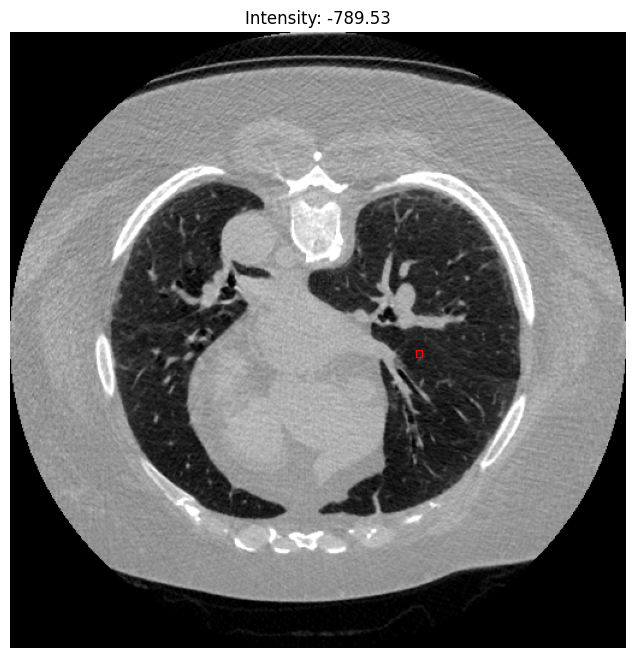
\includegraphics[width=0.6\linewidth]{images/non-visible-nodule-1.png}
    \caption{Example of a slice with an annotated nodule (at the indicated depth) that does not contain any visible tissue from the nodule itself. At the top the mean intensity expressed in Hounsfield Units (HU) of the area within the annotation. }
    \label{fig:non-visible-nodule}
\end{figure}

The strategy of extracting every 2D slice from a 3D volumetric bounding box is susceptible to annotation inaccuracies. Volumetric annotations are rarely perfect, often including slices at the superior and inferior extremes where the nodule is barely visible or entirely absent. Training the model on these ``empty" or noisy slices can introduce a significant amount of label noise, potentially degrading its performance by forcing it to learn from irrelevant or misleading examples.

To mitigate this, a dataset pruning strategy was developed to selectively remove these low-information slices. Several approaches were investigated to identify and remove them in a principled manner.

\subsubsection{Exploration of Pruning Strategies}
The core assumption behind our pruning is that slices containing predominantly healthy lung tissue or air will have a significantly lower average Hounsfield Unit (HU) intensity within the annotated bounding box compared to slices containing dense tumorous tissue. Based on this, the following strategies were explored:

\paragraph{Statistical Outlier Detection:} This initial approach, detailed in Algorithm \ref{alg:stat-pruning}, involved calculating the median ($\tilde{m}$) and Interquartile Range (IQR) of the mean bounding box intensities for all slices belonging to a single nodule. Slices with intensities considered to be low-end outliers were removed. However, this method proved to be overly aggressive, eliminating a substantial number of slices ($\sim$50\% of the dataset), including many that contained valuable information.

\begin{algorithm}[H]
    \caption{Strategy 1: Statistical Pruning}
    \label{alg:stat-pruning}
    \DontPrintSemicolon
    \SetAlgoLined
    \setstretch{1.2}

    \SetKwInOut{Input}{Input}
    \Input{
        SlicesForNodule: a list of (slice, mean\_intensity) pairs for one nodule\;
        $\alpha$: an adjustment factor (e.g., 1.5)
    }
    \SetKwData{keptSlices}{kept\_slices}
    \SetKwData{meanIntensities}{mean\_intensities}
    
    \BlankLine
    
    $\meanIntensities \gets$ [s.mean\_intensity for s in SlicesForNodule]\;
    Q1 $\gets$ FirstQuartile($\meanIntensities$)\;
    IQR $\gets$ InterquartileRange($\meanIntensities$)\;
    threshold $\gets$ Q1 - ($\alpha \times$ IQR)\;
    
    \BlankLine
    $\keptSlices \gets \{\}$\;
    \ForAll(){(slice, intensity) \textup{in} SlicesForNodule}{
        \If{intensity $\geq$ threshold}{
            $\keptSlices$.add(slice)\;
        }
    }
    \Return{$\keptSlices$}\;
\end{algorithm}


This approach, although being statistically sound, it tries to estimate properties of the mean intensity distribution, namely median and IQR, of each sample given a very limited number of slices for each nodule. This limitation often leads to an overly aggressive pruning, as the statistical estimates may not accurately reflect the true distribution of intensities.
It may also happen that if a given annotation is particularly noisy, shallow or generally mostly uninformative, the statistical properties of the mean intensity distribution may be skewed, leading to the opposite effect, removing informative slices as they might be detected as outliers of the distribution.

\paragraph{Sliding Window Approach:} To incorporate spatial locality, a sliding window of size $K$ was moved along the z-axis of each nodule (slices sorted by height). The window position that maximized the cumulative mean intensity was considered to contain the core of the nodule, as shown in Algorithm \ref{alg:sliding-window-pruning}. While this produced more coherent results, it was sensitive to the choice of $K$ and the full strategy (testing all possible values of $K$ and using an elbow method to choose the best one) proved overly complex.

\begin{algorithm}[H]
    \caption{Strategy 2: Sliding Window Pruning (fixed K)}
    \label{alg:sliding-window-pruning}
    \DontPrintSemicolon
    \SetAlgoLined
    \setstretch{1.2}
    
    \SetKwInOut{Input}{Input}
    \Input{
        SortedSlices: a list of slices for one nodule, sorted by z-index\;
        K: the size of the sliding window
    }
    \SetKwData{intensities}{intensities}
    \SetKwData{maxSum}{max\_sum}
    \SetKwData{bestStart}{best\_start\_index}

    \BlankLine
    
    $\intensities \gets$ [s.mean\_intensity for s in SortedSlices]\;
    $\maxSum \gets -\infty$\;
    $\bestStart \gets -1$\;
    
    \For{$i \gets 0$ \textup{to} len(SortedSlices) - K}{
        current\_sum $\gets$ Sum of $\intensities$ from index $i$ to $i+K-1$\;
        \If{current\_sum $>$ $\maxSum$}{
            $\maxSum \gets$ current\_sum\;
            $\bestStart \gets i$\;
        }
    }
    \Return{sub-list of SortedSlices from $\bestStart$ to $\bestStart+K-1$}\;
\end{algorithm}

Similarly to the statistical approach, this method ended up being overly aggressive, eliminating almost $40\%$ of the original data. This behaviour is due to the very shallow curve generated by the best cumulative mean intensity for each $K$. Meaning that the elbow point, supposed to indicate the optimal $K$ was often not well-defined. As a result, even when the annotation where well positioned, the method would still exclude some slices, although informative.
Nonetheless, the resulting dataset was definitely more coherent compared to the statistical approach.

\paragraph{Informed HU Thresholding:} The final and most effective strategy was a simple yet informed threshold, described in Algorithm \ref{alg:threshold-pruning}. Based on the typical HU values for soft tissue, a threshold of -750 HU was established. Any slice where the average intensity within the ground truth bounding box fell below this value was removed. This method is less aggressive and more clinically grounded, resulting in the exclusion of approximately 12.5\% of the total slices.

\begin{algorithm}[H]
    \caption{Strategy 3: Informed HU Thresholding}
    \label{alg:threshold-pruning}
    \DontPrintSemicolon
    \SetAlgoLined
    \setstretch{1.2}

    \SetKwInOut{Input}{Input}
    \Input{
        SlicesForNodule: a list of (slice, mean\_intensity) pairs for one nodule\;
        $T_{HU}$: the HU threshold (-750 HU)
    }
    \SetKwData{keptSlices}{kept\_slices}
    
    \BlankLine
    
    $\keptSlices \gets \{\}$\;
    \ForAll(){(slice, intensity) \textup{in} SlicesForNodule}{
        \If{intensity $\geq T_{HU}$}{
            $\keptSlices$.add(slice)\;
        }
    }
    \Return{$\keptSlices$}\;
\end{algorithm}

Despite its simplicity, this approach effectively balances the need to remove uninformative slices while preserving potentially informative ones.
Differently from the other methods, it does not need to estimate properties from the data distribution of a single nodule, but rather relies on established clinical knowledge about HU values, making it more robust to annotation noise and variability in nodule appearance.

\paragraph{Ablation Study Design}
To empirically validate the effectiveness of the final Informed HU Thresholding strategy, an ablation study was designed. The performance of the Faster R-CNN model will be compared across two experimental conditions:
\begin{itemize}
    \item \textbf{Baseline:} The model trained on the full dataset of all extracted slices.
    \item \textbf{Pruned:} The model trained on the dataset after applying the pruning strategy from Algorithm \ref{alg:threshold-pruning}.
\end{itemize}
This experiment was conducted using the EfficientNetV2-S backbone and the results of this ablation study are presented in Figure \ref{fig:threshold-pruning-ablation}.

\begin{figure}[h]
    \centering
    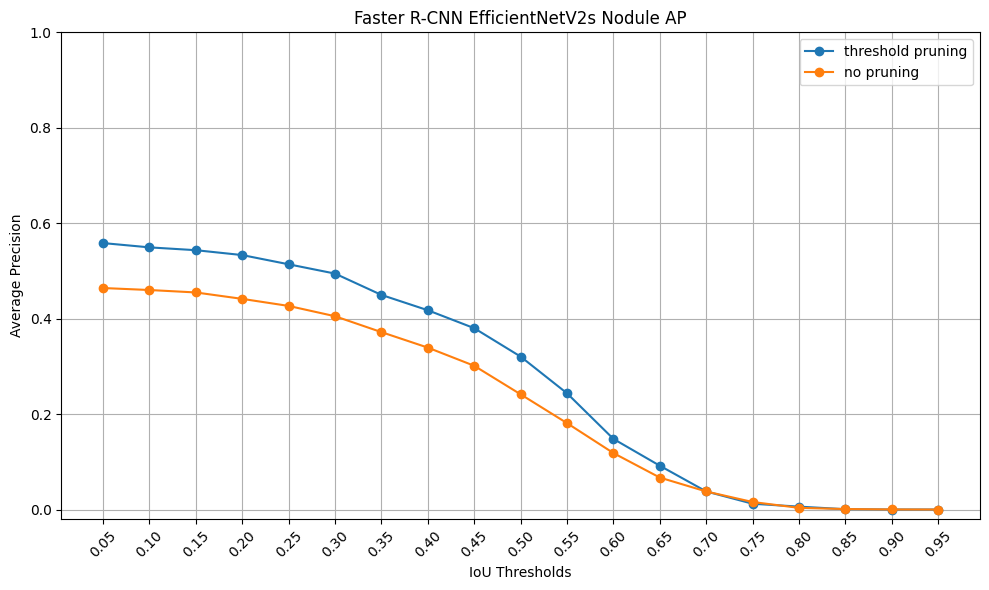
\includegraphics[width=0.8\linewidth]{images/threshold-pruning-ablation.png}
    \caption{Average Precision at varying IoU thresholds for threshold pruning ablation study.}
    \label{fig:threshold-pruning-ablation}
\end{figure}

The results clearly demonstrate the positive impact of the pruning strategy on the model's performance, particularly at higher IoU thresholds. This indicates that removing uninformative slices helps the model to focus on learning from relevant examples, thereby improving its detection capabilities. The Informed HU Thresholding strategy effectively enhances the quality of the training data, validating its inclusion in the preprocessing pipeline.\\

In addition to this ablation study, we also conducted a negative control experiment by training the same model on the dataset using the excluded slices only amounting to approximately 12.5\% of the original data ($\sim$1000 slices). The results of this experiment -- despite the limited amount of data -- showed an extremely poor performance, with an AP@5:95 of only 0.01, confirming that the excluded slices were indeed largely uninformative for the task of nodule detection.



\subsection{Three-channel Input Representation}
\label{sec:2.5d_approach}

While a 2D slice-based approach offers significant computational advantages over a full 3D analysis, it inherently discards the volumetric context that is crucial for accurate nodule characterization. In a single 2D slice, a small pulmonary nodule can be morphologically indistinguishable from a cross-section of a blood vessel or other anatomical structures. Radiologists naturally scroll through adjacent slices to observe how a feature evolves in the third dimension (the z-axis) to make a confident diagnosis.

To address this limitation without incurring the prohibitive memory and computational costs of full 3D convolutional networks, we adopt a multi-channel input representation, often referred to as a \textbf{2.5D approach}. This method synthesizes local volumetric information into a format that is directly compatible with standard 2D CNN architectures.
The idea comes from the observation that the pretrain used from ImageNet is on RGB images, which have already have three channels, while CT scans are single channel grayscale images, so we can leverage this by stacking adjacent slices to create a three-channel input, rather than copying the same slice three times.

For a given target slice at position $z$, which contains a nodule annotation, we construct a three-channel input tensor analogous to a standard RGB image. Instead of Red, Green, and Blue channels, the three channels are populated with grayscale intensity information from adjacent CT slices:

\begin{itemize}
    \item \textbf{Channel 1:} The preceding slice in the sequence, at position ($z-1$).
    \item \textbf{Channel 2:} The current target slice, at position ($z$).
    \item \textbf{Channel 3:} The subsequent slice in the sequence, at position ($z+1$).
\end{itemize}
If there is no available preceding or subsequent slice (e.g., at the beginning or end of a scan), the missing channel is filled by duplicating the target slice.
This technique offers several key advantages for our methodology:

\begin{itemize}
    \item \textbf{Enhanced Feature Representation:} It provides the model with crucial, localized 3D context. By seeing the preceding and subsequent slices, the network can learn to discern the characteristic spherical shape of a nodule as it changes across slices, helping to differentiate it from elongated, tubular structures like blood vessels.

    \item \textbf{Compatibility with Pre-trained Models:} It aligns perfectly with the three-channel input structure of the canonical backbone architectures used in this work (ResNet50, MobileNetV2, and EfficientNetV2-S). This allows for the direct and effective use of weights pre-trained on ImageNet, a dataset of three-channel RGB images, which is a cornerstone of modern transfer learning.

    \item \textbf{Computational Efficiency:} The approach processes three 2D slices at a time using standard 2D convolutions, thereby retaining the computational efficiency of a 2D pipeline. This avoids the exponential increase in parameters and memory usage associated with 3D convolutional layers, making the method accessible on commercial GPU hardware.
\end{itemize}

In cases where a preceding or subsequent slice is not available (i.e., for the very first or last slice in a nodule's sequence), the missing channel is populated by duplicating the target slice $z$. This padding technique ensures a consistent input dimension for all samples fed to the network.

\paragraph{Ablation Study Design:}
To empirically validate the effectiveness of the 2.5D approach, an ablation study was designed. The performance of the Faster R-CNN model will be compared across two experimental conditions:
\begin{itemize}
    \item \textbf{Single-channel Input:} The model trained using only the target slice as a single-channel grayscale image, with the channel duplicated to create a three-channel input.
    \item \textbf{Three-channel Input:} The model trained using the 2.5D approach, with the target slice and its adjacent slices forming a three-channel input. 
\end{itemize}
To conduct this study we used the Faster R-CNN model with an EfficientNetV2-S backbone on the DLCS dataset and the results are presented in Figure \ref{fig:3channel-ablation}.

\begin{figure}[h]
    \centering
    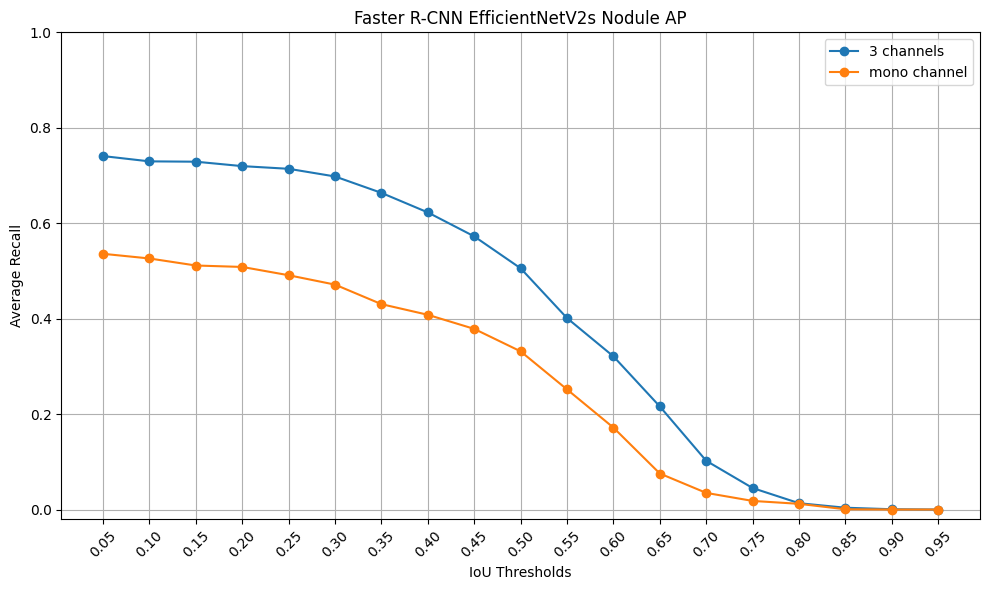
\includegraphics[width=.8\linewidth]{images/3-channel-ablation.png}
    \caption{Average Precision at varying IoU thresholds for 3-channel ablation study.}
    \label{fig:3channel-ablation}
\end{figure}

We can clearly see the impact that the 2.5D approach has on the model's performance, with a significant increase in Average Precision across all IoU thresholds when using the three-channel input representation. This demonstrates the value of incorporating local volumetric context into a 2D detection framework, validating the effectiveness of the 2.5D approach for pulmonary nodule detection. Given these results, the 2.5D three-channel input representation is adopted as the standard input format for all subsequent experiments in this thesis.

\section{Classification Dataset}
For the classification task, we derive a dataset from the DLCSD24 dataset, the only one of the two that contains both benign and malignant nodule annotations.
Each patch is labeled according to the malignancy of the nodule it contains, resulting in a binary classification problem (benign vs malignant).
The dataset is constructed by extracting patches around each annotated nodule, ensuring that the nodule is centered within the patch. Before any extraction takes place, each CT-Scan undergoes the same preprocessing pipeline described in Section \ref{sec:preprocessing}, including resampling to a uniform voxel size and HU clipping.
The classes of this dataset are highly imbalanced, with a ratio of approximately 1:10 between benign and malignant nodules. To address this imbalance during training, we employ an oversampling strategy, where benign nodules are cloned a number of times in the dataset to match the number of malignant nodules. This approach help to ensure that the model is exposed to a balanced representation of both classes during training, which is crucial to prevent bias towards the majority class and to improve the model's ability to generalize to unseen data.

\subsection{Additional Preprocessing for Classification}
In addition to the preprocessing steps outlined in Section~\ref{sec:preprocessing}, the classification dataset requires further preprocessing to ensure that the input patches are of a consistent size and format suitable for training a classification model.

\subsubsection{Panning and Resizing}
The classification dataset is constructed by extracting zoomed-out patches centered around each annotated nodule. The reason behind this choice is to provide the classification model with sufficient contextual information about the nodule's surroundings, and to ensure that the nodule is fully contained within the patch, accounting for potential annotation's inaccuracies. The size of these patches is determined based on the specific nodule size, ensuring that smaller nodules are not lost in overly large patches, while larger nodules are fully captured.
To achieve this, we first determine the bounding box of each nodule based on its annotation. We then expand this bounding box by 80\% in both width and height to create a zoomed-out view that includes surrounding tissue.
This expansion factor was chosen empirically to balance the need for context with the desire to keep the nodule as the focal point of the patch.
An important choice is the aspect ratio of the extracted patches. In this work, we experimented with both square patches (1:1 aspect ratio) and by keeping the original aspect ratio of the bounding box. The importance of this choice is due the need of resizing the extracted patches to a fixed size, a necessary step due to the presence of a fully-connected layer at the end of the CNN architecture. Such resizing, would introduce a distortion in the nodule's shape if the original aspect ratio is preserved -- due its variability --, a problem that is avoided by using square patches. However, this comes at the cost of potentially including a significant amount of irrelevant background in the patch, especially for nodules with extreme aspect ratios. 
To decide which approach to use, we conducted an ablation study.

\paragraph{Ablation Study Design:}
To empirically validate the impact of patch aspect ratio on classification performance, an ablation study was designed. The performance of the classification model will be compared across two experimental conditions:
\begin{itemize}
    \item \textbf{Square Patches:} The model trained using square patches (1:1 aspect ratio) resized to a fixed size of $512\times512$ pixels.
    \item \textbf{Original Aspect Ratio Patches:} The model trained using patches that preserve the original aspect ratio of the bounding box, resized to a fixed size of $512\times512$ pixels. 
\end{itemize}

%results of the ablation study

A padding approach has been considered to resize the original aspect ratio patches to a square shape without distortion, by adding black borders to the shorter side of the patch. However, this approach was ultimately not adopted as smaller nodules would end up being surrounded by a significant amount of black space, and most of the model's ``attention'' would be focused on this irrelevant area, hindering its ability to learn meaningful features from the nodule itself.    